%\addbibresource{/home/jorgsk/phdproject/bibtex/jorgsk.bib}
The aim for this doctoral work was to use computational tools in combination
with empirical experiments to study regulation of gene expression due to
variation in DNA sequences. This culminated in using calculations of free
energy changes for base pairing of RNA and DNA molecules to study transcription
initiation and translation initiation.

RNA and DNA molecules are polymers nucleotides denoted by G, A, C, and T (U
instead of T for RNA). Due to their polymer nature RNA and DNA are also called
nucleotide chains. It is today taken for granted that these nucleotide chains
can anneal together by base pairing to form complementary double stranded DNA
and RNA, as well as RNA-DNA hybrids.  However, these double stranded nucleotide
chains deserve our attention since they are essential for the replication
of DNA, for the synthesis of RNA through transcription, and for the synthesis
of protein through translation.  Nucleotide base pairing therefore makes up the
foundation for how cells make use of and replicate the genetic information.

The role of double stranded DNA in DNA replication is made clear by the famous
quote from the study by Watson and Crick from their discovery of the structure
of double stranded DNA, "(...) the specific pairing we have postulated
immediately suggests a possible copying mechanism for the genetic material"
\cite{watson_molecular_1953}. In other words, that the DNA helix consists of
two complementary molecules enables the accurate base-to-base replication of
the genetic material that is necessary for the propagation of life the way we
know it.

In transcription, base pairing plays its role through the ~9/10 length RNA-DNA
hybrid that is formed within the RNA polymerase. During RNA synthesis, each new
RNA nucleotide must first bind to template DNA before a phosphodiester bond
binds it to the rest of the RNA chain, and thereby to the RNA-DNA hybrid. This
ensures that RNA is a faithful base-to-base copy of the genetic information in
DNA.

In translation, RNA-RNA base pairing is necessary to build the amino acid chain
of proteins. One part of this pairing is the thee-nucleotide codons on mRNA and
the other part is the complementary anticodon of the tRNA that carries the next
amino acid of the chain. Other biological processes which depend on base
pairing include the formation of secondary and tertiary structures of folded
RNA; micro-RNA regulation by hybridization to full-length RNA; and the binding
of the 16S RNA of the bacterial ribosome to the Shine-Dalgarno sequence of
messenger RNA (mRNA) to initiate protein synthesis.

In addition to these evolved roles, many lab-technical uses and assays have
been found that exploit nucleotide chain base pairing or hybridization. One
example is PCR, which relies on the temperature-dependence of DNA helix
formation, which is exploited for opening and closing double stranded DNA.
Another example is gene silencing, in which small interfering RNA (siRNA) can
be constructed to base pair with coding regions of mRNA to interfere with
protein synthesis. Yet a third example is the DNA microarray, which relies on
constructing optimal RNA probes for hybridizing with the target DNA sequence.

Regardless of the biological function mediated by nucleotide base pairing, the
function can be greatly influenced by the strength of the base pairing. In
general, GC-rich sequences form stronger base pairs than sequences that
are AT-rich. It is however relatively unknown that the cause for the variation
in binding strength is only partially due to hydrogen bonding (3 bonds for GC
and 2 bonds for AT) and primarily due to different stacking of the GC and AT
nucleotides \cite{yakovchuk_base-stacking_2006}. Look-up tables for the
strength of RNA-DNA, DNA-DNA, and RNA-RNA dinucleotide pairs are available in
the literature, and have a long history of use in computational biology,
especially in the field of predicting RNA secondary structures
\cite{mathews_prediction_2006}.

In the main work in this thesis I have used calculations of the binding
strengths of DNA-DNA bonds (of double stranded DNA) and RNA-DNA bonds (of the
RNA-DNA hybrid) (as well as other free energies) to investigate the
translocation of RNA polymerase (RNAP) relative to DNA immediately after
transcription initiation. This enabled the discovery of an association between
RNAP translocation and abortive RNA synthesis from failed promoter escape
attempts. Based on this finding, transcription initiation experiments were
performed which supported the computational findings. This has resulted in new
knowledge about the relationship between the initial transcribed DNA sequence
and promoter escape in bacteria and is the major result of this thesis.

In a different type of study, I have calculated RNA secondary structures using
methods that rely on RNA-RNA base pairing to predict how the secondary
structures affect the binding of the bacterial ribosome to mRNA. By
experimentally testing sequences with different secondary structures, these
calculations aided investigations that centered around improving protein
expression systems.

In addition to these studies, which were performed at the NTNU in Trondheim, I
had the opportunity to spend a year working with a project at the lab of Dr.
Roderic Guigó at the Centre for Genomic Regulation in Barcelona. The work I
performed there involved the analysis of nucleotide sequences; however, instead
of using free energies, I focused on analysing poly(A) sequences in
high-throughput RNA sequencing (RNA-seq) data to study pre-RNA processing in
the form of cleavage and polyadenylation. This work has broadened the view of
the thesis by investigating the regulation of gene expression from a
genome-wide perspective, as opposed to the gene-centric approach of the two
first studies.

Seen as a whole, the work in this thesis centers around different aspects of
gene expression: transcription initiation, translation initiation, and pre-RNA
processing. This is illustrated in Figure \ref{fig:thesis_visual}. On the left
in this figure on can see the aspects of gene expression that have been
studied, and on the right can be found the main computational methods that have
been used to study them.

An interesting contrast in this work is the two different strategies that have
been used to study the different aspects of expression: for the studies with
free energy and secondary structure, a traditional gene-centric,
single-molecule approach has been used; while for the study of 3\ppp cleavage
and polyadenylation a top-down genome wide approach has been taken. The
utilization of these two different approaches, which can also be referred to as
hypothesis-driven and data-driven, will make up part of the final discussion at
the end of the thesis.

The following sections of the introduction consist of reviews of both the
biological phenomena in Figure \ref{fig:thesis_visual} and the computational
methods.

\begin{figure}[htb]
	\begin{center}
		\includegraphics[scale=0.6]{illustrations/thesis_visual_abstract_portrait.pdf}
	\end{center}
	\caption{}
	\label{fig:thesis_visual}
\end{figure}
